\documentclass[]{article}
\usepackage[utf8]{inputenc}
\usepackage[left = 1.5cm, right = 1.5cm, top = 2cm, bottom = 2cm]{geometry}

\usepackage{graphicx}
\usepackage{float}
\usepackage{amsmath}
\usepackage{cleveref}
\usepackage{minted}
\usepackage{color}

\begin{document}

	\begin{titlepage}
	\begin{center}
		\vspace*{1cm}
		
		\Huge
		\textbf{PV Measurement}
		
		\vspace{0.5cm}
		\LARGE
		48550 Renewable Energy Systems - Lab 1
		
		\vspace{1.5cm}
		
		\textbf{Robert Carey}\space\space\space99139382\\
		\textbf{William Rooke}\space\space\space 12051342\\
		\textbf{Joel Goodwin}\space\space\space 98055953\\
		
		\today
		
		\vfill
		
		
		\vspace{0.8cm}
		
		\includegraphics[width=1\textwidth]{uts}
		
		
		
	\end{center}
\end{titlepage}
	
	\tableofcontents
	\newpage
	\listoffigures
	\newpage
	\section{Introduction}
		The purpose of this report is to develop two Maximum Power Point Tracking (MPPT) algorithms, Constant Voltage Reference and Perturb and Observe, for use in a solar photovoltaic (PV) renewable energy system. In place of a functional PV panel, a PV emulator, consisting of a string of diodes, is used in order to make the experiments easier to conduct and the algorithms easier to troubleshoot.

	 	
 	\section{Constant Voltage Reference MPPT}
		\subsection{Pre-Work}
 			\subsubsection{Explain the working principle of the PV emulator.}
				\begin{figure}[H]
					\centering
					\includegraphics*[width=0.75\textwidth]{Prework_images/PVDiagram}
					\caption{Diagram of PV emulator and voltage control}
				\end{figure}
				It can be seen from the above diagram that
				\begin{equation}\label{eq:TotalCurrent}
					I_{pv} = I_{ph} - i_{Dpv} - i_p
				\end{equation}
				where the diode current $i_{Dpv}$ is given by
				\begin{equation}\label{eq:DiodeCurrent}
					i_{Dpv} = I_S (e^{\frac{V_D}{V_T}} - 1)
				\end{equation}
				and the thermal voltage of the diode $V_T$ is 
				\begin{equation}\label{eq:ThermalVoltage}
					V_T=\frac{K_B*T*A}{q}
				\end{equation}
				where A is the ideality factor of the solar cell, q is the charge of an electron, $K_B$ is the Boltzmann constant, T is the temperature in Kelvin and the voltage across the diode $V_D$ is
				\begin{equation}\label{eq:DiodeVoltage}
					V_D=V_{pv\_c}-I_{pv}*R_s
				\end{equation}
				The leakage current $I_p$ is given by
				\begin{equation}\label{eq:LeakageCurrent}
					i_p=\frac{V_{pv\_c}+I_{pv}*R_s}{R_{sh}}
				\end{equation}
				Combining \crefrange{eq:TotalCurrent}{eq:LeakageCurrent} gives the output current as
				\begin{equation}
					I_{pv}=I_{ph}-I_S(e^\frac{V_{pv\_c}-I_{pv}*R_s}{\frac{K_B*T*A}{q}}-1)-\frac{V_{pv\_c}+I_{pv}*R_s}{R_{sh}}
				\end{equation}
				As $R_{sh}$ does not affect the output voltage and is comparatively large compared to $R_s$, it can be ignored. Therefore, the power of the system is given by $P=I*V_{pv\_c}$ or
				\begin{equation}
					P=V_{pv\_c}*(I_{ph}-I_S(e^\frac{V_{pv\_c}-I_{pv}*R_s}{\frac{K_B*T*A}{q}}-1))
				\end{equation}
				The equation parameters $I_s$, $I_{ph}$ and $R_s$ can either found experimentally or from technical literature.
				\\
				The simulated PV emulator and the I-V and P-V curves from LTSpice are shown in \cref{fig:LTSpice,fig:IVCurve}
				\begin{figure}[H]
					\centering
					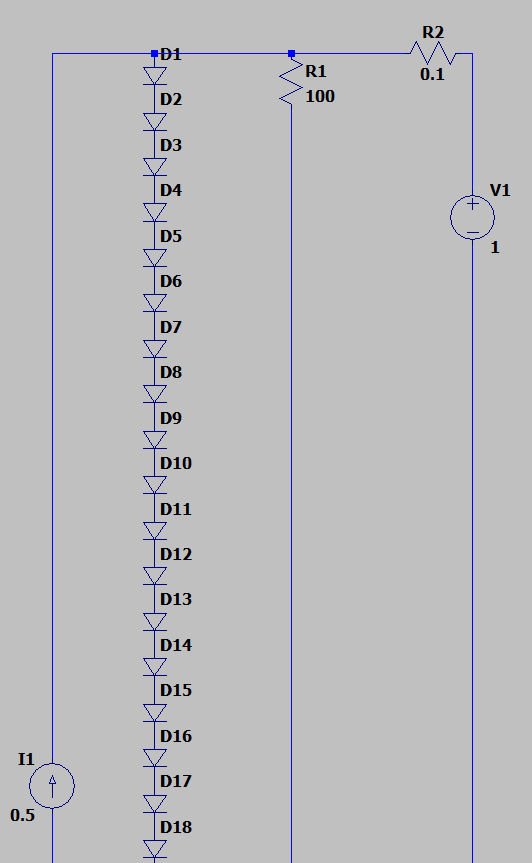
\includegraphics[width=0.5\textwidth]{Prework_images/LTSpice_cropped}
					\caption{PV emulator LTSpice circuit}
					\label{fig:LTSpice}
				\end{figure}
			 	\begin{figure}[H]
			 		\centering
					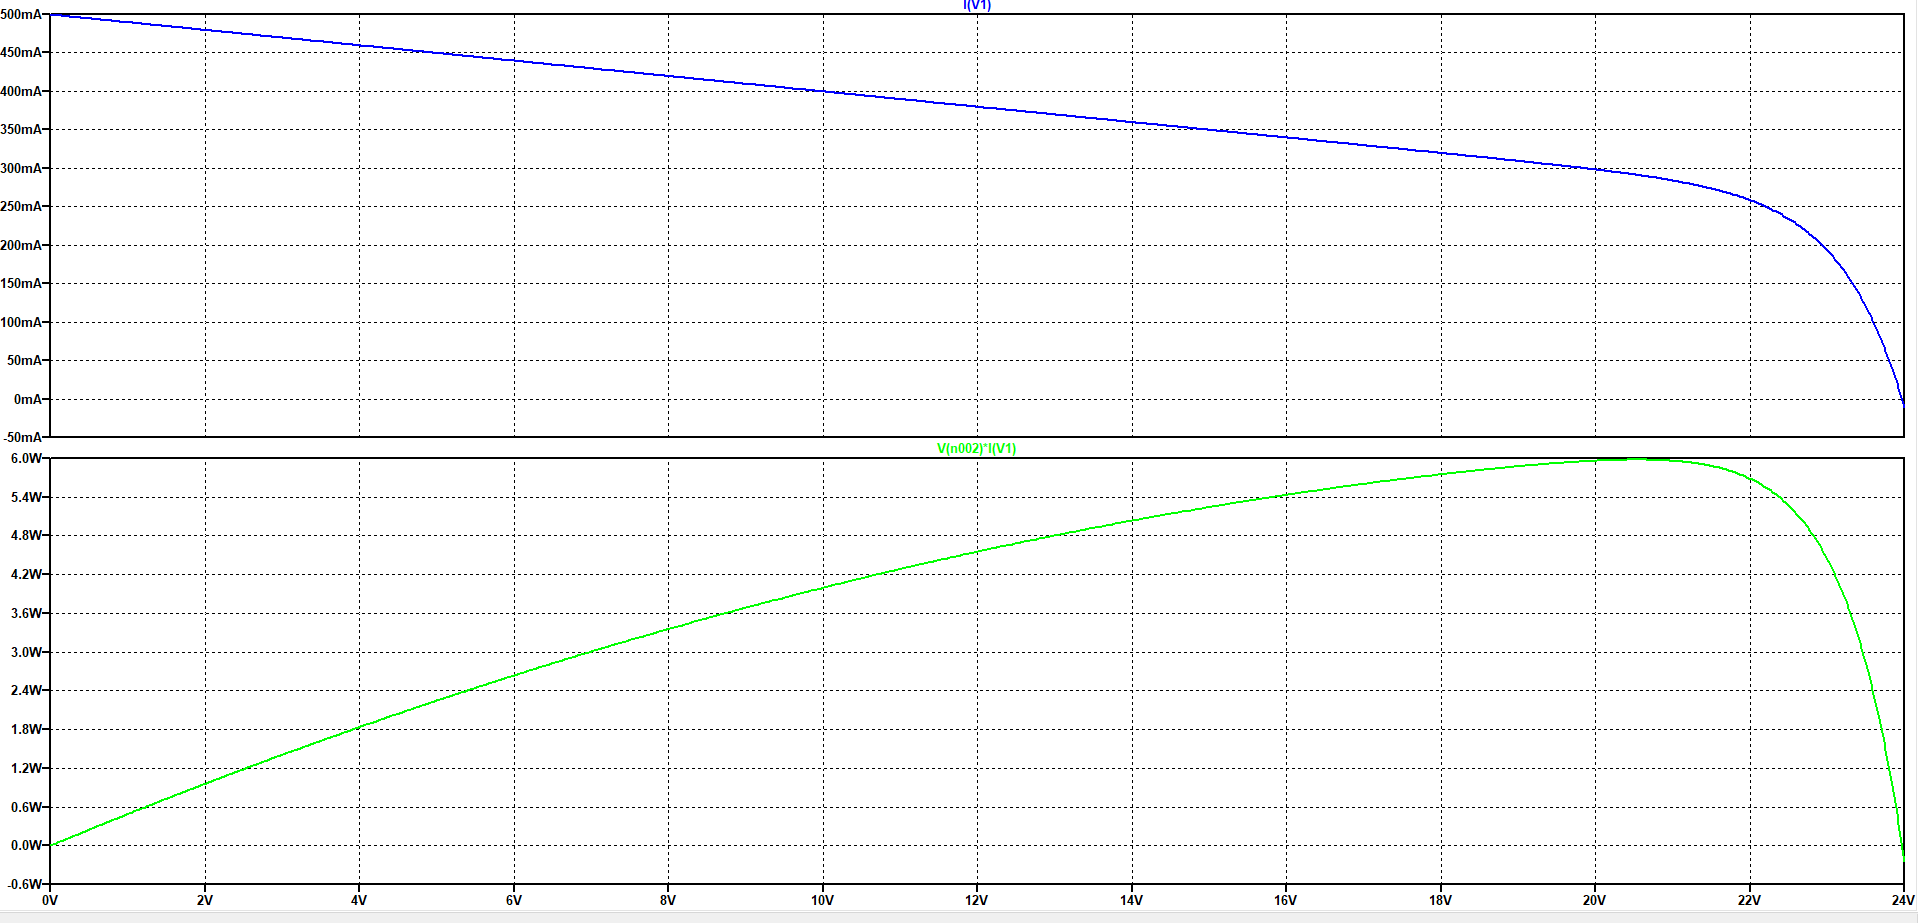
\includegraphics[width=\textwidth]{Prework_images/IVCurve}
					\caption{I-V and P-V curves of LTSpice PV emulator}
					\label{fig:IVCurve}
				\end{figure}
			\subsubsection{Explain how the duty cycle should change to make the PV panel voltage constant and operate at the reference}
				If the PV panel voltage drops below the reference value, the duty cycle should be decreased in order to bring the voltage back to the reference value. Similarly, if the PV voltage rises above the reference value, the duty cycle should be increased to ensure the PV voltage drops to the reference voltage.
				
		\subsection{Lab Work}
			\subsubsection{PV Emulator}\label{sssec:PVEmu}
				In order to properly implement the constant voltage reference MPPT algorithm, the maximum power point of the PV emulator was found by connecting the PV emulator in parallel with the lab power supply and connecting a variable resistance box to the circuit. The resistance was changed between $0\Omega$ and $270\Omega$ and the voltage and current were measured. Open circuit conditions were also measured. The results are shown in \cref{tbl:Lab3Emu}, and the I-V and P-V curves are shown in \cref{fig:Lab3IV,fig:Lab3PV}
				\begin{table}[H]
					\centering
					\begin{tabular}{|l|l|l|l|}
						\hline												
						Resistance & Current & Voltage & Power \\ \hline
						0 & 0.412 & 0.22 & 0.09064 \\ \hline
						1 & 0.411 & 0.7 & 0.2877 \\ \hline
						4.7 & 0.411 & 2.17 & 0.89187 \\ \hline
						10 & 0.411 & 4.34 & 1.78374 \\ \hline
						22 & 0.41 & 9 & 3.69 \\ \hline
						33 & 0.409 & 13.3 & 5.4397 \\ \hline
						47 & 0.396 & 18.5 & 7.326 \\ \hline
						68 & 0.313 & 20.9 & 6.5417 \\ \hline
						100 & 0.208 & 20.9 & 4.3472 \\ \hline
						220 & 0.095 & 20.9 & 1.9855 \\ \hline
						245 & 0.085 & 20.9 & 1.7765 \\ \hline
						270 & 0.077 & 20.9 & 1.6093 \\ \hline
						O/C & 0 & 20.9 & 0 \\ \hline												
					\end{tabular}
					\caption{Electrical characteristics of PV emulator}
					\label{tbl:Lab3Emu}
				\end{table}
				\begin{figure}[H]
					\centering
					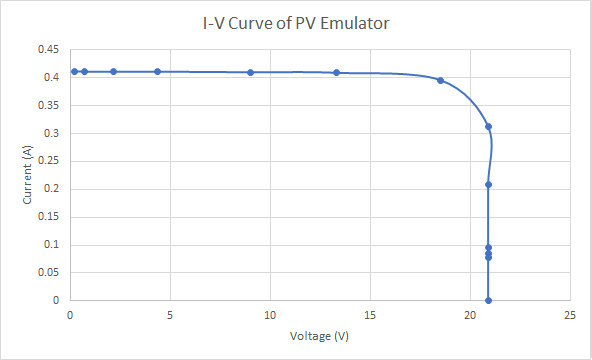
\includegraphics[width=0.75\textwidth]{Lab3Results/IVCurve}
					\caption{I-V curve of PV emulator}
					\label{fig:Lab3IV}
				\end{figure}
				\begin{figure}[H]
					\centering
					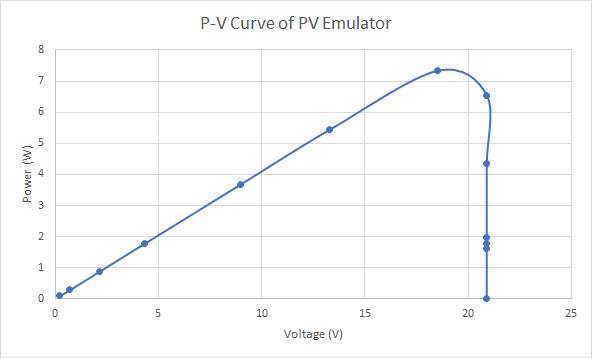
\includegraphics[width=0.75\textwidth]{Lab3Results/PVCurve}
					\caption{P-V curve of PV emulator}
					\label{fig:Lab3PV}
				\end{figure}
			
			\subsubsection{Testing of Constant Voltage Reference MPPT}\label{sssec:CVRMPPT}
				The lab's buck converter was connected between the PV emulator and the variable resistance box, and set up using an Arduino as the PWM driver. The lab power supply was set to 21V and the resistance box set to $33\Omega$. It was verified to be operating correctly, as shown in \cref{fig:lab3buck}.
				\begin{figure}[H]
					\centering
					\includegraphics[width=0.75\textwidth]{Lab3Results/BuckTest_50DutyCycle_100KHz}
					\caption{Correct operation of lab buck converter}
					\label{fig:lab3buck}
				\end{figure}
				The MPPT algorithm could then be tested by varying the input current and measuring the output power. Oscilloscope captures showing the duty cycle of the buck converter, displayed in orange, power output of the buck converter, displayed in pink, the input current, displayed in blue, and output voltage, displayed in red, are shown in \crefrange{fig:Lab3_0.3A}{fig:Lab3_0.6A}
				\begin{figure}[H]
					\centering
					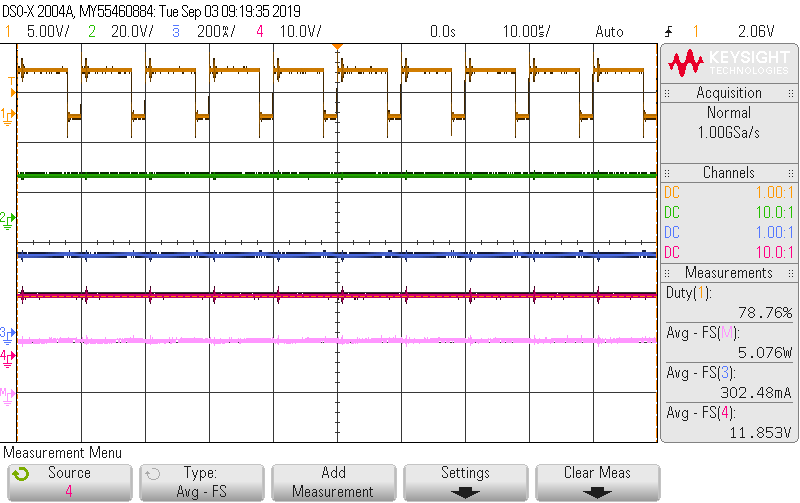
\includegraphics[width=0.75\textwidth]{Lab3Results/0_30A_Supply}
					\caption{Constant Voltage Reference MPPT with 0.3A supply}
					\label{fig:Lab3_0.3A}
				\end{figure}
				\begin{figure}[H]
					\centering
					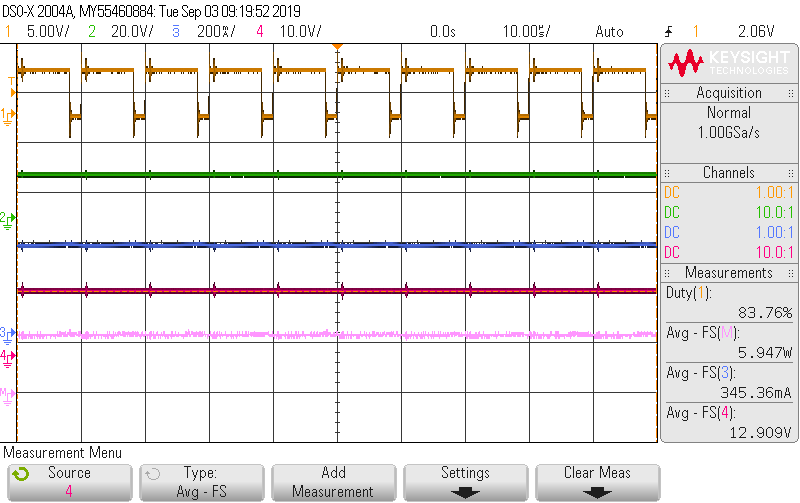
\includegraphics[width=0.75\textwidth]{Lab3Results/0_35A_Supply}
					\caption{Constant Voltage Reference MPPT with 0.35A supply}
					\label{fig:Lab3_0.35A}
				\end{figure}
				\begin{figure}[H]
					\centering
					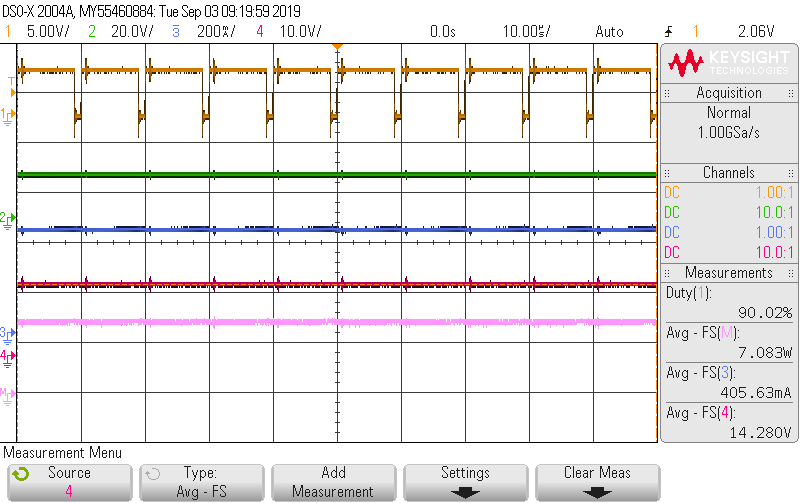
\includegraphics[width=0.75\textwidth]{Lab3Results/0_40A_Supply}
					\caption{Constant Voltage Reference MPPT with 0.4A supply}
					\label{fig:Lab3_0.4A}
				\end{figure}
				\begin{figure}[H]
					\centering
					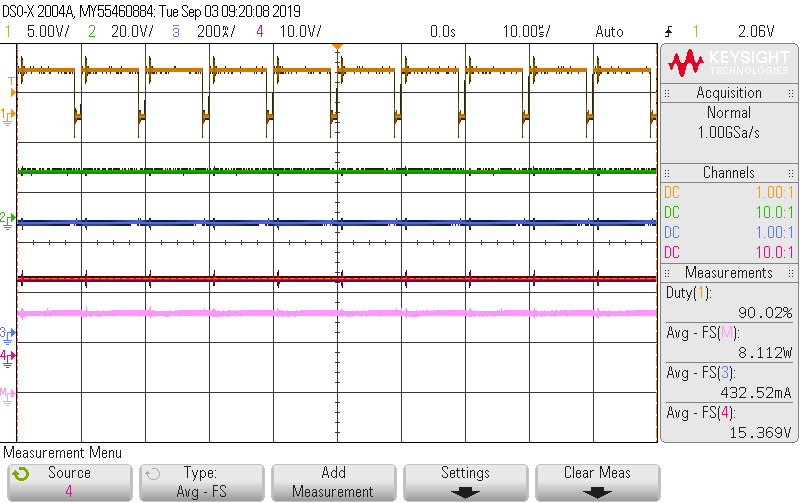
\includegraphics[width=0.75\textwidth]{Lab3Results/0_45A_Supply}
					\caption{Constant Voltage Reference MPPT with 0.45A supply}
					\label{fig:Lab3_0.45A}
				\end{figure}
				\begin{figure}[H]
					\centering
					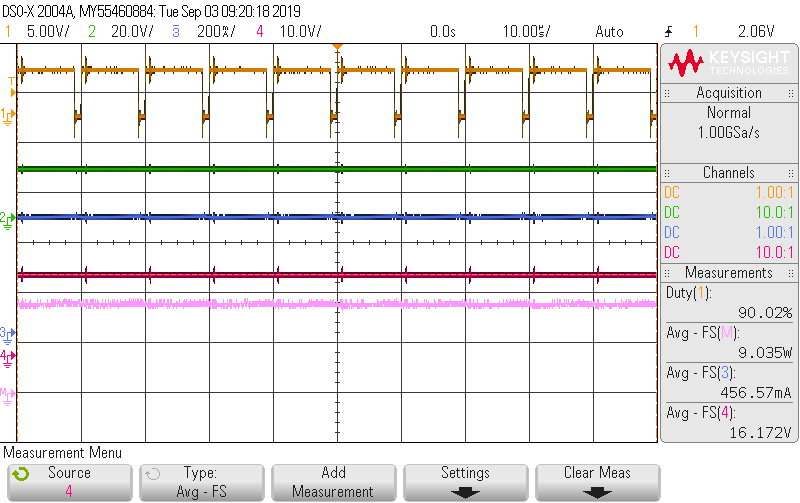
\includegraphics[width=0.75\textwidth]{Lab3Results/0_50A_Supply}
					\caption{Constant Voltage Reference MPPT with 0.5A supply}
					\label{fig:Lab3_0.5A}
				\end{figure}
				\begin{figure}[H]
					\centering
					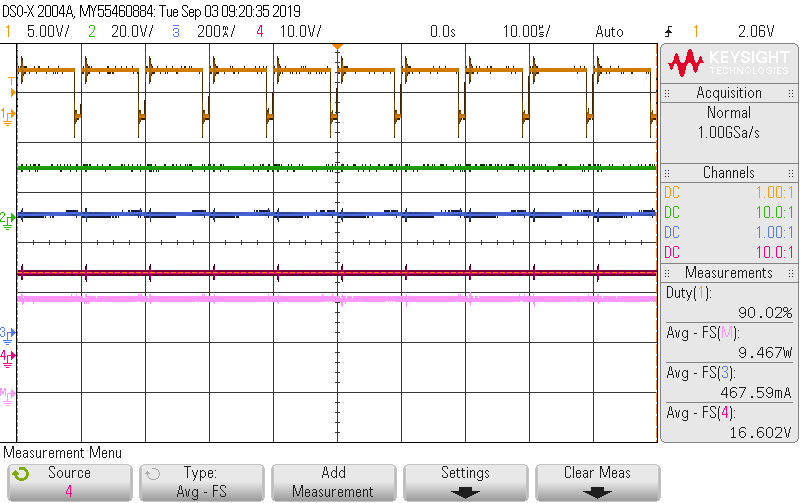
\includegraphics[width=0.75\textwidth]{Lab3Results/0_55A_Supply}
					\caption{Constant Voltage Reference MPPT with 0.55A supply}
					\label{fig:Lab3_0.55A}
				\end{figure}
				\begin{figure}[H]
					\centering
					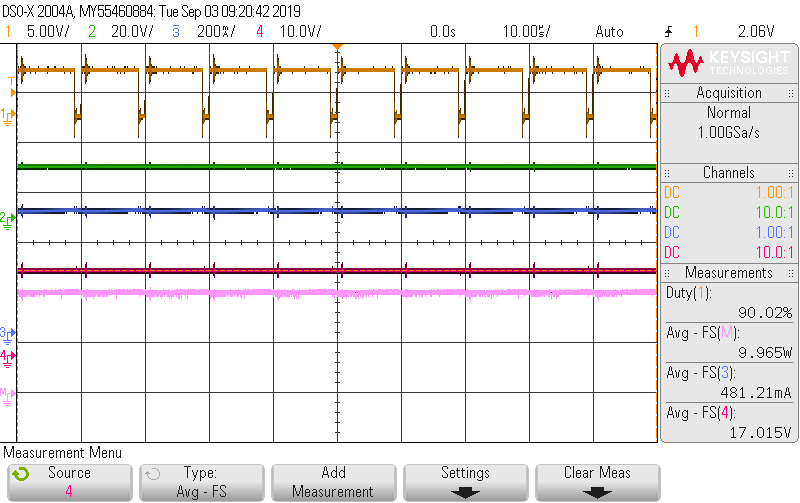
\includegraphics[width=0.75\textwidth]{Lab3Results/0_60A_Supply}
					\caption{Constant Voltage Reference MPPT with 0.6A supply}
					\label{fig:Lab3_0.6A}
				\end{figure}
		\newpage
 		\subsection{Analysis}
 			\subsubsection{Explain, with aid of equations and diagrams, how the buck converter serves as a variable resistor to the PV panel} 			
 				The electric power for the system is given by 				
 				\begin{equation*}
 					V_o I_o = \eta V_i I_i
 				\end{equation*}
 				where $V_o$ and $I_o$ are the output voltage and current, $\eta$ is the efficiency of the system, and $V_i$ and $I_i$ are the input voltage and current. Using Ohm's Law, $I_o$ and $I_i$ can be represented as
 				\begin{align*}
 					I_o = \frac{V_o}{Z_o}\\
 					I_i = \frac{V_i}{Z_i}
 				\end{align*}
 				where $Z_o$ and $Z_i$ are the output and input impedances. Substituting these into the previous equation results in
 				\begin{equation*}
 					\frac{V_o^2}{Z_o}=\frac{\eta V_i^2}{Z_i}
 				\end{equation*}
 				Assuming the buck converter is operating in continuous mode, $V_o = DV_i$, where $D$ is the duty cycle, meaning that
 				\begin{align*}
 					\frac{V_o^2}{Z_o}=\frac{\eta V_i^2}{Z_i}\\
 					\implies\frac{(DV_i)^2}{Z_o}=\frac{\eta V_i^2}{Z_i}
 				\end{align*}
 				This can be simplified to
 				\begin{equation*}
 					\frac{D^2}{Z_o}=\frac{\eta}{Z_i}
 				\end{equation*}
 				and further to
 				\begin{equation*}
 					D = \sqrt{\frac{\eta Z_o}{Z_i}}
 				\end{equation*}
 				This shows that the changing the duty cycle of the buck converter effectively changes the impedance ratio seen by the source, acting as a variable resistor.
 				
			\subsubsection{Explain your part of the code to achieve constant voltage reference MPPT with the support of experimental results}
				\begin{listing}[H]
					\begin{minted}[autogobble]{cpp}
						convVolt = analogRead(pin_ADC) * 0.0049;
						adjVoltage = convVolt / 0.18;
						Serial.println(adjVoltage);
						if (adjVoltage > vref)
							Duty = Duty + 1;
						else if (adjVoltage < vref)
							Duty = Duty - 1;
						if (Duty > 90)
							Duty = 90;
						else if (Duty < 10)
							Duty = 10;
					\end{minted}
					\caption{Code for Constant Voltage Reference MPPT}
					\label{lst:CVR}
				\end{listing}
				The method of operation for the Constant Voltage Reference MPPT can be seen in \cref{lst:CVR}. The Arduino initially reads a voltage from the output of the buck converter, then converts and adjusts it so it is represented as a true voltage. This input voltage is then compared against the reference voltage \mintinline{cpp}{vref}. If the input voltage is greater than the reference, the duty cycle is increased to lower the input voltage. If the input voltage is less than the reference, the duty cycle is decreased to increase the input voltage. The code also limits the duty cycle such that it remains between 10\% and 90\% to prevent damage to the buck converter.
				
 			\subsubsection{Compare the constant voltage reference MPPT performance against the identified true MPPs}
	 			Unfortunately, when gathering the I-V and P-V curves for the PV emulator in \cref{sssec:PVEmu}, only one set of data with a current limit of 400mA was taken, meaning the performance of the MPPT algorithm cannot be shown across different insolation levels. However, in \cref{fig:Lab3_0.4A}, it can be seen that the output power is approximately 7W, close to the maximum power point identified in \cref{fig:Lab3PV}. It is possible that the algorithm could have tracked closer to the MPP, however the duty cycle of the buck converter being limited to 90\% may have prevented this.
	\newpage
 	\section{Perturb and Observe (P\&O) MPPT}
		\subsection{Pre-Work}
			\subsubsection{Explain why the power information at a particular point can be simplified to:\\$\text{Power information at point } X = V_{out} \times V_{PV}$} \label{sssec:Powerinfo}
				The power of the PV panel is given by $P_{PV} = I_{PV} \times V_{PV}$, where $I_{PV}$ is the current and $V_{PV}$ is the voltage produced by the PV panel. As the current produced by the PV panel can be found by multiplying the circuit output current, $I_{out}$, by the duty cycle of the buck converter, $D$, the power equation can be represented as $P_{PV} = D I_{out} \times V_{PV}$. Using Ohm's Law, the equation can be further represented as $P_{PV} = D \frac{V_{out}}{R_{out}} \times V_{PV}$. As the P\&O algorithm does not need to take actual values into account, only their relative magnitudes, any constant values can be omitted and the power information can be represented as:
				\begin{equation*}
					\text{Power information at point } X = V_{out} \times V_{PV}
				\end{equation*}
 							
				
			\subsubsection{Design a Perturb and Observe Algorithm in Your Own Words}
			The control system obtains the power information at a given point on the PV panel's P-V curve using the equation in \cref{sssec:Powerinfo} and stores it. The control system then reduces the buck converter's duty cycle and measures the power information at the new operating point. If the power at the new operating point is greater than the old operating point, the control system will continue to decrease the duty cycle when measuring the change. However, if the power information at the new operating point is less than that at the old operating point, the control system will increase the duty cycle. Once the power begins to drop again, the control system will start to decrease the duty cycle. This process happens continuously, ensuring the power output will oscillate around the maximum power point of the system.\\
 					
			Overall, when the power drops when the duty cycle is increasing, the controller will switch to decreasing the duty cycle, and if the power drops while the duty cycle is decreasing, the controller will switch to increasing the duty cycle.
			 
		\subsection{Lab Work}
			\subsubsection{PV Emulator}
				In order to test the P\&O MPPT algorithm, the MPPs of the PV emulator were found in a similar fashion to \cref{sssec:PVEmu}. The PV emulator was tested with current limits of 400, 300 and 200 mA. The results are shown in \crefrange{tbl:lab4_400emu}{tbl:lab4_200emu} and the I-V and P-V curves are shown in \cref{fig:lab4IVCurve,fig:lab4PVCurve}
				\begin{table}[H]
					\centering	 				
					\begin{tabular}{|l|l|l|l|}
						\hline	 					
						Resistance & Current & Voltage & Power \\ \hline
						0 & 0.39 & 0.064 & 0.02496 \\ \hline
						1 & 0.39 & 0.46 & 0.1794 \\ \hline
						4.7 & 0.39 & 1.9 & 0.741 \\ \hline
						10 & 0.39 & 4.14 & 1.6146 \\ \hline
						22 & 0.39 & 8.7 & 3.393 \\ \hline
						33 & 0.396 & 12.87 & 5.09652 \\ \hline
						47 & 0.38 & 18.76 & 7.1288 \\ \hline
						68 & 0.305 & 20.85 & 6.35925 \\ \hline
						100 & 0.204 & 20.86 & 4.25544 \\ \hline
						220 & 0.091 & 20.87 & 1.89917 \\ \hline
						245 & 0.082 & 20.87 & 1.71134 \\ \hline
						270 & 0.074 & 20.87 & 1.54438 \\ \hline
						O/C & 0 & 20.86 & 0 \\ \hline			 					
					\end{tabular}
			 		\caption{Electrical characteristics of PV emulator at 400mA current limit}
			 		\label{tbl:lab4_400emu}
				\end{table}
				\begin{table}[H]
					\centering
					\begin{tabular}{|l|l|l|l|}
						\hline		 					
						Resistance & Current & Voltage & Power \\ \hline
						0 & 0.308 & 0.05 & 0.0154 \\ \hline
						1 & 0.308 & 0.36 & 0.11088 \\ \hline
						4.7 & 0.308 & 1.47 & 0.45276 \\ \hline
						10 & 0.308 & 3.22 & 0.99176 \\ \hline
						22 & 0.307 & 6.76 & 2.07532 \\ \hline
						33 & 0.306 & 10 & 3.06 \\ \hline
						47 & 0.304 & 15.5 & 4.712 \\ \hline
						68 & 0.276 & 19.35 & 5.3406 \\ \hline
						100 & 0.203 & 20.87 & 4.23661 \\ \hline
						220 & 0.09 & 20.87 & 1.8783 \\ \hline
						245 & 0.082 & 20.87 & 1.71134 \\ \hline
						270 & 0.074 & 20.88 & 1.54512 \\ \hline
						O/C & 0 & 20.88 & 0 \\ \hline		 					
					\end{tabular}
					\caption{Electrical characteristics of PV emulator at 300mA current limit}
					\label{tbl:lab4_300emu}
				\end{table}
 				\begin{table}[H]
 					\centering
 					\begin{tabular}{|l|l|l|l|}
 						\hline	 						
 						Resistance & Current & Voltage & Power \\ \hline
 						0 & 0.201 & 0.123 & 0.024723 \\ \hline
 						1 & 0.201 & 0.238 & 0.047838 \\ \hline
 						4.7 & 0.201 & 0.96 & 0.19296 \\ \hline
 						10 & 0.201 & 2.1 & 0.4221 \\ \hline
 						22 & 0.2 & 4.4 & 0.88 \\ \hline
 						33 & 0.2 & 6.5 & 1.3 \\ \hline
 						47 & 0.2 & 9.86 & 1.972 \\ \hline
 						68 & 0.198 & 13.6 & 2.6928 \\ \hline
 						100 & 0.182 & 18.6 & 3.3852 \\ \hline
 						220 & 0.09 & 20.9 & 1.881 \\ \hline
 						245 & 0.082 & 20.9 & 1.7138 \\ \hline
 						270 & 0.074 & 20.9 & 1.5466 \\ \hline
 						O/C & 0 & 20.9 & 0 \\ \hline	 						
 					\end{tabular}
		 			\caption{Electrical characteristics of PV emulator at 200mA current limit}
		 			\label{tbl:lab4_200emu}
 				\end{table}
				\begin{figure}[H]
					\centering
					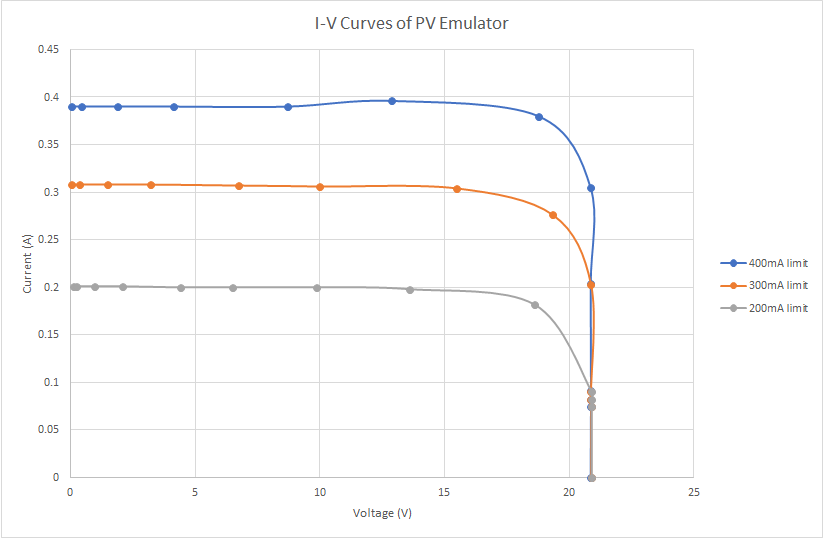
\includegraphics[width=0.75\textwidth]{Lab4Results/IV_Curve}
					\caption{I-V curves of PV emulator}
					\label{fig:lab4IVCurve}
				\end{figure}
	 			\begin{figure}[H]
	 				\centering
	 				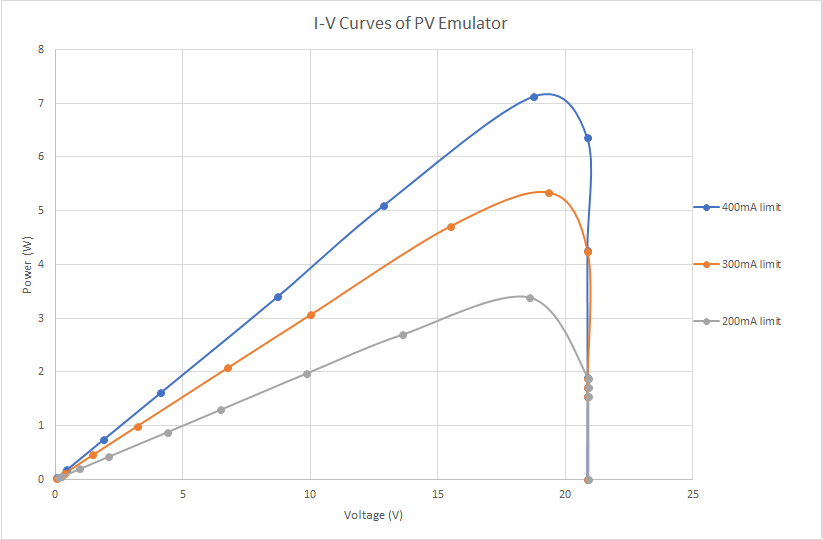
\includegraphics[width=0.75\textwidth]{Lab4Results/PV_Curve}
	 				\caption{P-V curves of PV emulator}
	 				\label{fig:lab4PVCurve}
	 			\end{figure}
 			\subsubsection{Testing of P\&O MPPT Algorithm}
 				The P\&O MPPT algorithm was tested in a similar fashion to the Constant Voltage Reference MPPT algorithm in \cref{sssec:CVRMPPT}. Once, the buck converter was verified to be working correctly, shown in \cref{fig:lab4buck}, the new algorithm was tested. In the results shown, the duty cycle of the buck converter is shown in orange, the power output of the system is shown in pink, the input current is shown in blue and the output voltage is shown in red.
 				\begin{figure}[H]
 					\centering
 					\includegraphics[width=0.75\textwidth]{Lab4Results/BuckTest_50DutyCycle_100KHz}
 					\caption{Correct operation of lab buck converter}
 					\label{fig:lab4buck}
 				\end{figure}
 				
 				The results are shown in \crefrange{fig:Lab4_0.3A}{fig:Lab4_0.5A}
 				\begin{figure}[H]
 					\centering
 					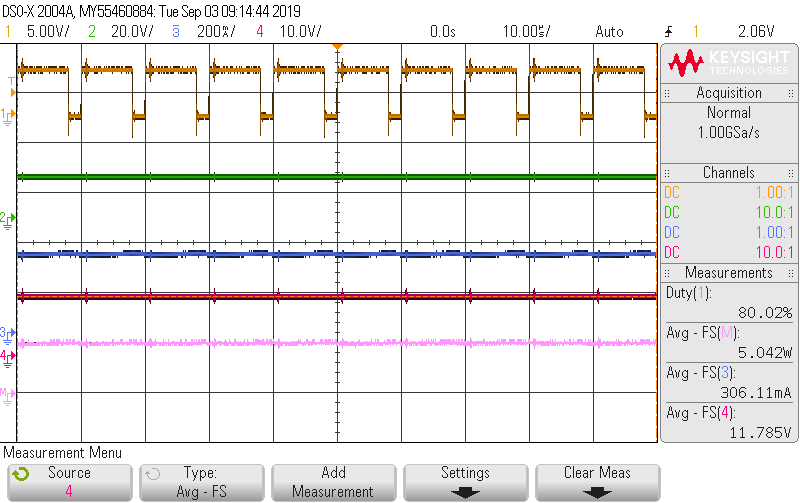
\includegraphics[width=0.75\textwidth]{Lab4Results/0_30A_Supply}
 					\caption{Perturb and Observe MPPT with 0.3A supply}
 					\label{fig:Lab4_0.3A}
 				\end{figure}
 				\begin{figure}[H]
 					\centering
 					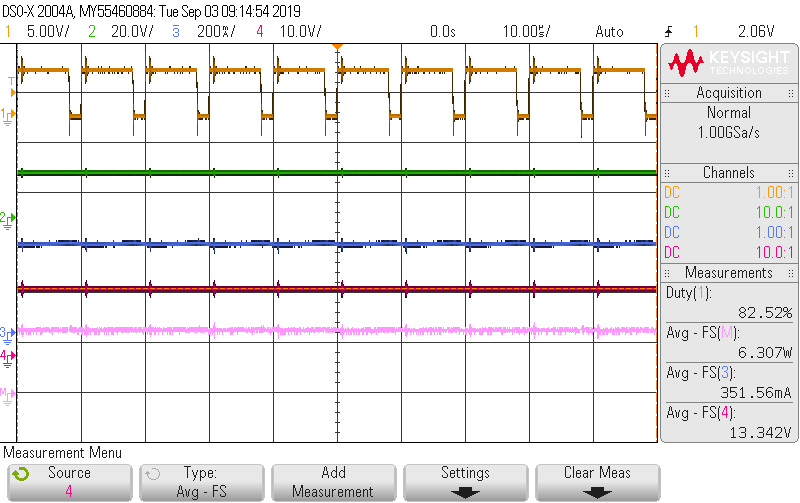
\includegraphics[width=0.75\textwidth]{Lab4Results/0_35A_Supply}
 					\caption{Perturb and Observe MPPT with 0.35A supply}
 					\label{fig:Lab4_0.35A}
 				\end{figure}
 				\begin{figure}[H]
 					\centering
 					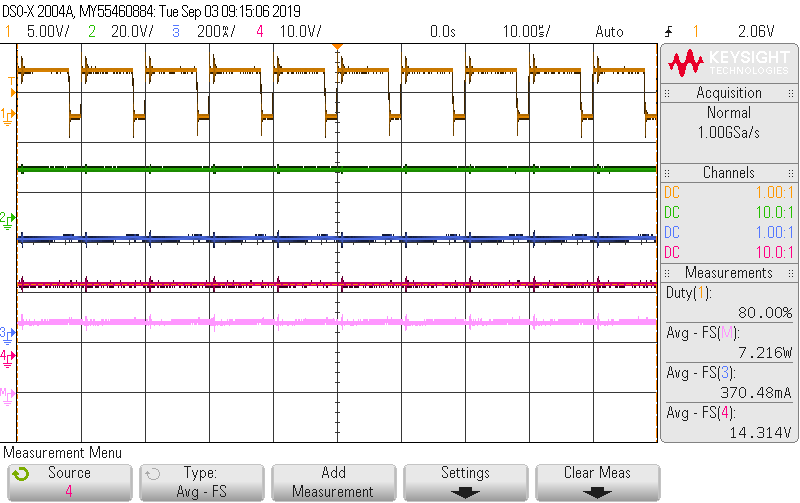
\includegraphics[width=0.75\textwidth]{Lab4Results/0_40A_Supply}
 					\caption{Perturb and Observe MPPT with 0.4A supply}
 					\label{fig:Lab4_0.4A}
 				\end{figure}
 				\begin{figure}[H]
 					\centering
 					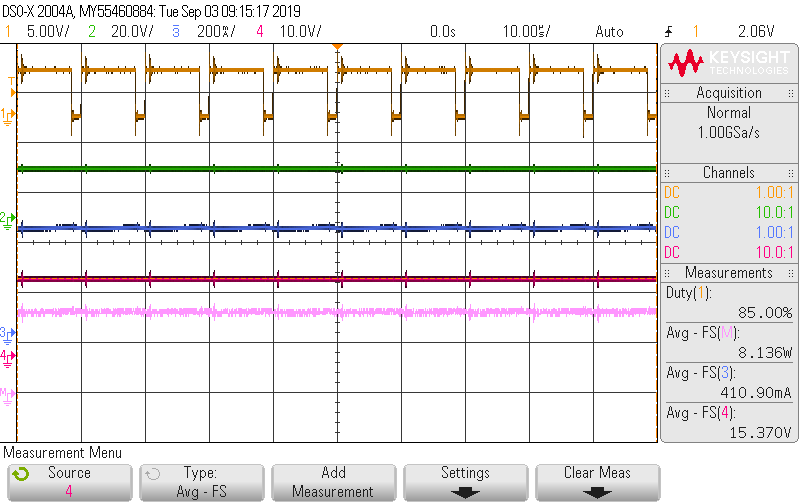
\includegraphics[width=0.75\textwidth]{Lab4Results/0_45A_Supply}
 					\caption{Perturb and Observe MPPT with 0.45A supply}
 					\label{fig:Lab4_0.45A}
 				\end{figure}
 				\begin{figure}[H]
 					\centering
 					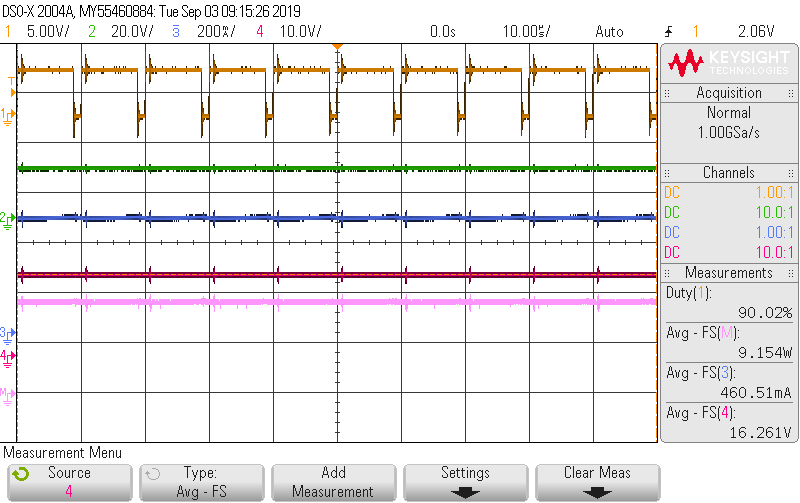
\includegraphics[width=0.75\textwidth]{Lab4Results/0_50A_Supply}
 					\caption{Perturb and Observe MPPT with 0.5A supply}
 					\label{fig:Lab4_0.5A}
 				\end{figure}
 		\newpage
 		\subsection{Analysis}
 			\subsubsection{Explain your part of the code to achieve P\&O MPPT with the support of experimental results}
 				\begin{listing}[H]
 					\begin{minted}[autogobble]{cpp}
	 					Vout_CV = analogRead(ADC_Vout) * 0.0049;
	 					Vout_adjV = Vout_CV / 0.18;
	 					Vpv_CV = analogRead(ADC_Vpv) * 0.0049;
	 					Vpv_adjV = Vpv_CV / 0.18;
	 					
	 					newP = Vout_adjV * Vpv_adjV;
	 					
	 					if (oldP > newP)
	 						Duty = Duty - 1;
	 					else
	 						Duty = Duty + 1;
	 					
	 					if (Duty > 90)
	 						Duty = 90;
	 					else if (Duty < 10)
	 						Duty = 10;
	 					
	 					setDutyCycle(Duty);
	 					oldP = newP;	 					
 					\end{minted}
 					\caption{Code for Perturb and Observe MPPT}
 					\label{lst:MPPT}
 				\end{listing}
 				The algorithm initially reads the output and the PV emulator voltages, then adjusts and converts them to values representing the real voltages. It then multiplies these values to get the power information at that point, as explained in \cref{sssec:Powerinfo}, completing the Observe phase of the algorithm. This power information is then compared with the old power information; if the new power is greater than the old power, the duty cycle is reduced; whereas if the new power is less than the old power, the duty cycle is increased. This completes the Perturb phase of the algorithm. The new power is then considered the old power and stored for use in the next cycle of the algorithm.
 				
 			\subsubsection{Compare the P\&O MPPT performance against the identified true MPPs}
 				It can be seen from \cref{fig:lab4PVCurve} that the MPPs exist at approximately 7.2W and 5.4W for 400mA and 300mA current limits respectively. The experimental results shown in \cref{fig:Lab4_0.4A,fig:Lab4_0.3A} show that the power points the algorithm tracked to are approximately equal to the MPPs at the given current limits.
 			\subsubsection{Is P\&O a perfect maximum power point algorithm? Why or why not? Explain your argument with the experimental results if possible}
 				Perturb and Observe could be considered a near-perfect MPPT algorithm due to the ease of which it tracks to the maximum power point. Its performance, however, depends greatly on the size of the disturbance used in the Perturb phase of the algorithm. If the disturbance is too large, the algorithm will never be able to reach the MPP of the system due to large, constant oscillation. Similarly, if the disturbance is too low, the algorithm may not be fast enough to cope with changing insolation conditions. Both of these scenarios result in reduced efficiency levels and, as such, the size of the disturbance used must be closely considered.
 			\subsubsection{Suggest a way to improve the tracking accuracy of P\&O}
 				Using an adaptive disturbance would improve the tracking accuracy of the P\&O algorithm. The size of the disturbance used in the Perturb phase of the algorithm would change depending on whether the algorithm was close to the MPP or not. If the current power point is far from the maximum, the disturbance size would be larger than if the maximum had already been reached. This would allow the MPP to be found faster while still maintaining a high level of efficiency when the MPP has been found.
\end{document}

